%--------------------------------------------------------
%--------------------------------------------------------
\comment{How does the radial kernel reduce to unity on evaluating the the operator on to its inverse ? This will be important to understand how to define alternate radial functions.}
\section{Generalized operators}
The azimuthal dependence of the convolution kernels which translate the Stokes parameters Q \& U to the scalar E \& B is determined by the spin properties of the field being operated upon and the spin of the resultant fields. Hence there is no freedom in the choice of function for the azimuthal dependence of the convolution kernels. The radial part of the function however is determined by the choice of the basis functions.  It is possible to generalize these convolution kernels by choosing alternate forms for the radial functions.

We can characterize different forms of the radial kernel by introducing the following harmonic space operator,
%
\beq
\tilde{\mathcal{G}} = {\begin{bmatrix} g_{\ell}^E & 0  \\  0 & g_{\ell}^B \end{bmatrix}} \,,
\eeq
%
where the functions $g_{\ell}^E$ and $g_{\ell}^B$ represent the harmonic representation of the modified radial functions and can in the most general case be chosen to be different for E and B modes. To simplify the discussion and without loosing this generality we proceed with the assumption $g_{\ell}^E = g_{\ell}^B= g_{\ell}$. We can chose this function to be any arbitrary function and it will allow us to define some convolution operator which either translates Stokes Q \& U parameters to scalars E \& B or vice verse. Given $\tilde{\mathcal{G}}$ the modified forward and inverse convolution kernels are given by the following expressions,
%
\begin{subequations} \label{eq:gen_qu2eb}
\beqry
{\bar O}' &=& {{}_0\mathcal{Y}} *\tilde T^{-1}*\tilde{\mathcal{G}}* {{}_2\mathcal{Y}^{\dagger}} *\bar T \,,\\
{\bar O}'^{-1}&=& \bar{T}^{-1} *{{}_2\mathcal{Y}}* \tilde{\mathcal{G}}^{-1} *\tilde T *{{}_0\mathcal{Y}^{\dagger}}
\eeqry
\end{subequations}
%
where we have used the primed notation  to distinguish these generalized operators from the default operators defined in \sec{sec:qu2eb} and \sec{sec:eb2qu}. Note that for an arbitrary choice of $\tilde{\mathcal{G}}$ only one of the operators in \eq{eq:gen_qu2eb} is well defined, since $\tilde{\mathcal{G}}^{-1}$ may be ill defined. If we require both the forward and inverse hold true, then we are constrained in choosing $\tilde{\mathcal{G}}$ such that its inverse is well defined.

The radial part of these generalized convolution kernels is now given by the following expressions,
%
\begin{subequations}
\beqry
G_{QU \rightarrow EB}(\beta) &=& G(\beta) = \sum _{\ell=2} ^{\ell_{\rm max}} g_{\ell}\frac{2 \ell+1}{4 \pi} \sqrt{\frac{(\ell-2)!}{(\ell + 2)!}} P_{\ell}^2(\cos{\beta}) \, \label{eq:mod_rad_forward} \\
G_{EB \rightarrow QU}(\beta) &=& G^{-1}(\beta) = \sum _{\ell=2} ^{\ell_{\rm max}} g_{\ell}^{-1}\frac{2 \ell+1}{4 \pi} \sqrt{\frac{(\ell-2)!}{(\ell + 2)!}} P_{\ell}^2(\cos{\beta}) \,,\label{eq:mod_rad_inverse}
\eeqry
\end{subequations}
%
where $g_{\ell}$ are the same multipole function as those appearing in $\tilde{\mathcal{G}}$. If one chooses different forms of $g_{\ell}$ for E and B modes then the radial function are defined accordingly. Given this general definition for the radial function $G(\beta)$, note that the default radial function $f(\beta)$ is just a special case resulting from the choice $\tilde{\mathcal{G}}=\tilde{\mathcal{I}}$ ($g_{\ell}=1$). Note that for this choice of $\tilde{\mathcal{G}}$ the inverse is trivial $\tilde{\mathcal{G}}^{-1}=\tilde{\mathcal{G}}$ and therefore $G^{-1}(\beta) = G(\beta)$.

While defining these alternate operators by modifying the radial part of the kernels, it seems more natural to make a choice on the real space function $G(\beta)$ as compared to choosing the multipole function $g_{\ell}$. Using the orthogonality property of associated Legendre polynomials it can be shown that the multipole function $g_{\ell}$ is given by the following integral over the radial function $G(\beta)$,
%
\beq
g_{\ell} = 2 \pi \sqrt{\frac{(\ell-2)!}{(\ell+2)!}} \int _{0}^{\pi} G(\beta) P_{\ell}^{2}(\cos{\beta}) d\cos{\beta} \,. \label{eq:gb2bl}
\eeq
%
Here it is important to note that the radial function $G(\beta)$ has to be chosen such that it vanishes at $\beta=0$ and $\beta=\pi$. One way to understand this is that the associated Legendre polynomials $P_{\ell}^2 \propto \sin^2{\beta}$ vanish at these values of the abscissa and hence cannot be used to describe functions which don't have this property.  Another way to understand this requirements is that at these locations the coordinate dependence of the Stokes parameters cannot be integrated out, since the azimuthal angle is ill defined and hence the convolution kernel needs to have vanishing contribution from these locations. \revisit{The normalization of these functions is not critically important, since any choice defines a convention. It is important to ensure consistency with the convention once a choice has been made.} \comment{find a better location for this}

In contrast to the radial function $G(\beta)$ an instrumental beam function appropriately normalized has the property $B(\beta) \rightarrow 1$ as $\beta \rightarrow 0$. A circularly symmetric beam is represented in harmonic space by the multipole function $b_{\ell}$ which can be derived by evaluating the coefficients of expansion of the function $B(\beta)$ defined at the pole in the Legendre polynomial $P_{\ell}^0$ basis. The effective instrument beam is \revisit{almost} always identical for $E$ and $B$ modes. \comment{Distinguishing E/B localization characterized by $g_{\ell}$ from E/B smoothing characterized by $b_{\ell}$.}
%
\beq
B(\beta) = \sum_{\ell=0}^{\ell_{\rm max}} \frac{2 \ell+1}{4 \pi} b_{\ell} P_{\ell}^{0} (\cos{\beta})\,,
\eeq
%
\comment{A co-polarized beam which measures the Stokes parameters is not the same as a smoothing beam measuring a scalar field. Is it important to discuss the polarization beam details here ?}
%
\begin{figure}[!t] 
\centering
\subfigure[\label{fig:bl_gbeta}]{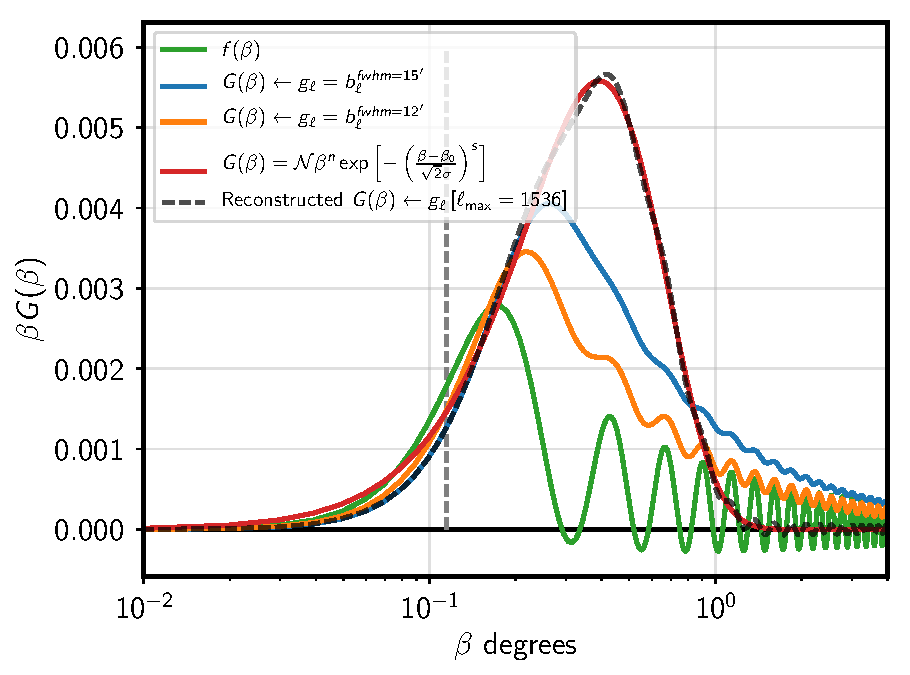
\includegraphics[width=0.32\columnwidth]{Gbeta_for_different_gl_lmax1536.pdf}}
\subfigure[]{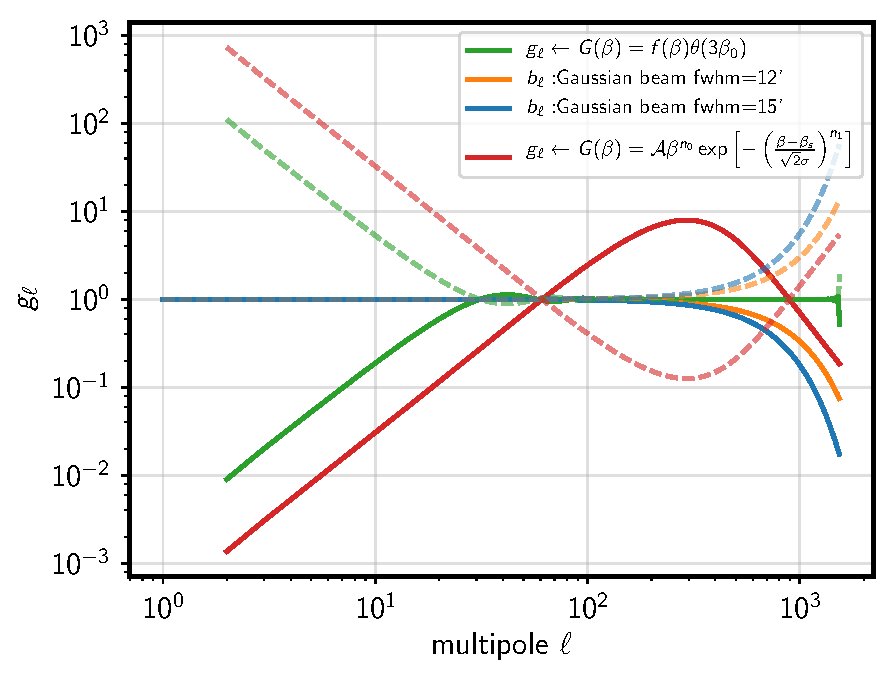
\includegraphics[width=0.32\columnwidth]{gl_for_different_gbeta_lmax1536.pdf}}
\subfigure[\label{fig:gl_bbeta}]{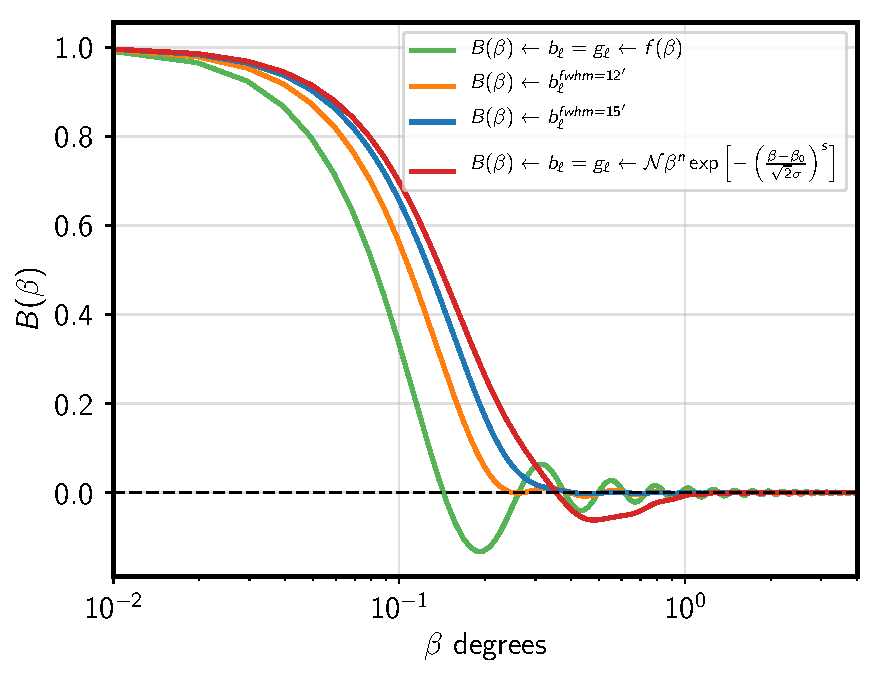
\includegraphics[width=0.32\columnwidth]{Bbeta_for_gl_lmax1536.pdf}}
\caption{\textit{Left:} The vertical dashed gray line depicts the approximate pixel size $\Delta_{\rm pix} = \sqrt{\frac{4 \pi}{N_{\rm pix}}}$ of a Nside=512 Healpix map. The green line depicts the default radial kernel $f(\beta)$ defined in \eq{eq:qu2eb_gen_kernel}. The blue and orange lines depict the modified radial function resulting the beam harmonics $b_{\ell}$ corresponding to Gaussian beams with fwhm=15 \& 12 arcminutes respectively. The red curve depicts an example modified radial function: $G(\beta)=\mathcal{N} \beta^n \exp{\left[ -\left( \frac{\beta-\beta0}{\sqrt{2} \sigma} \right)^s \right]}$ with parameters set to the following values $[n=1;\, \beta_0=0 ;\, \sigma = 2\Delta_{\rm pix} ;\, s=1.5]$. The black dashed curve depicts the band limited reconstruction of the modified radial function $G(\beta)$. We intentionally have plotted $\beta G(\beta)$ to clearly depict the high $\beta$ behavior of these functions. \textit{Middle: } This figure depicts the harmonic representation of the respective radial functions as indicated by the legend. The dashed curves of the corresponding color depict the inverse of the harmonic functions. \textit{Right:} This figure depicts the beam function $B(\beta)$ evaluated from interpreting the respective harmonic functions as those corresponding to an instrument beam.}
\label{fig:example_gbeta}
\end{figure}
%
Though the real space behavior of these two function $G(\beta)$ and $B(\beta)$ has important differences, in harmonic space they play identical roles. Therefore it is possible to interpret the beam harmonic coefficients as those representing some modified radial kernel. The modified radial kernel resulting from a few example Gaussian beams are depicted in \fig{fig:bl_gbeta}.
it is possible to interpret the harmonic representation $g_{\ell}$ of the radial function $G(\beta)$ as those corresponding to some circularly symmetric instrument beam function. The beam function corresponding to the default radial kernel and the modified radial kernel $G(\beta)$ are depicted in \fig{fig:gl_bbeta}.

\comment{Move the following two paragraphs to final discuss}
\revisit{The discussion till now gives the impression that using the localized convolution kernels is no different from from using the default kernel and altering the spherical harmonic coefficients of expansion of the relavant fields by appropriately operating on them with the  effective beam functions $g_{\ell}$. To appreciate the difference between these two, it is important to realize that in general one can make a choice of a radial function which may not have a band limited description. In such a case these two method of evaluating the relevant fields is not identical. An example of this claim is depicted in \fig{fig:example_gbeta}.\\
Another important thing to realize is that the harmonic coefficients derived from default full sky operations get some contributions from different portions of sky. For instance evaluating the E and B fields in the vicinity of the poles is are prone to receiving significant contributions from strong foregrounds near the equator. Correcting the harmonic coefficients of expansion with the effective beam function does not cancel these non-local contribution. On the contrary by performing the convolution with the localized real space kernels, the regions which contribute to the local field evaluations are predetermined by the choice of the radial function.} 


%In \sec{sec:local_conv_eb} we constructed localized convolution kernels by multiplying $R(\beta)$ with an apodized version of the step function $\theta_{\rm apo}(r_{\rm cutoff})$. The oscillation seen in the spectra in \fig{fig:eb-spectra_rad_cutoff} can be explained to be due to this effective beam characterized by $g_{\ell}^2$ operating on the power spectra. The effective beam can be evaluated by computing the multipole function $g_{\ell}$ as follows,
%%
%\beq
%g_{\ell} = 2 \pi \sqrt{\frac{(\ell-2)!}{(\ell+2)!}} \int _{0}^{r_{\rm cutoff}} R(\beta) \theta_{\rm apo}(r_{\rm cutoff})  P_{\ell}^{2}(\cos{\beta}) d\cos{\beta} \,, \label{eq:gb2bl} \,,
%\eeq
%%
%where the upper limit of the integration is set to $r_{\rm cutoff}$ since the function $\theta_{\rm apo}(r_{\rm cutoff})$ vanishes for $\beta>r_{\rm cutoff}$. The function $b^2_{\ell}-1$ matches the oscillation seen in \fig{fig:eb-spectra_rad_cutoff} as  seen in \fig{fig:match_cl_oscillations} where the two results have been over plotted.
%%
%\begin{figure}[!t] 
%\centering
%\subfigure[]{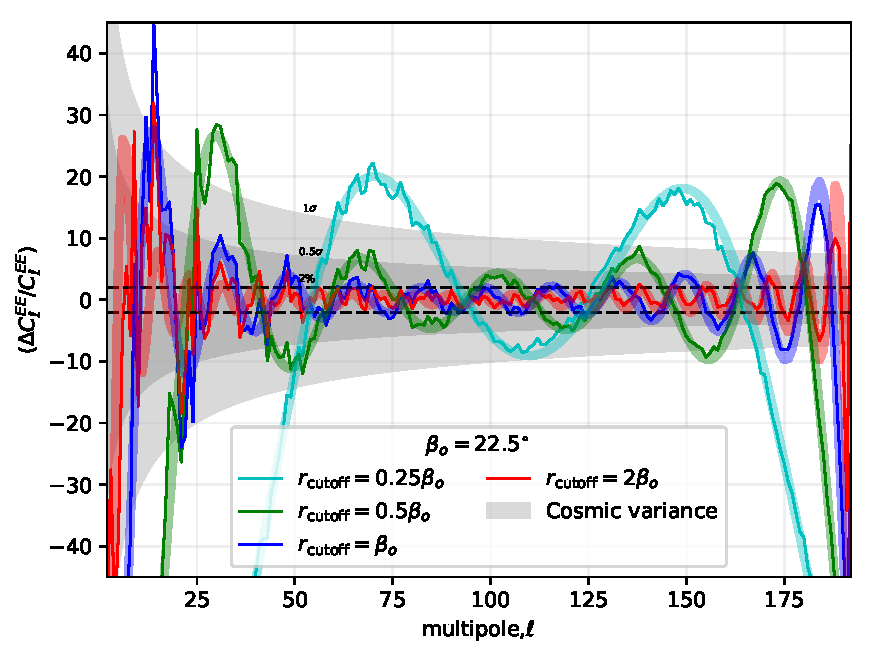
\includegraphics[width=0.98\columnwidth]{analytical_cl_oscillations_vs_data.pdf}}
%\caption{The thin lines depicts the same spectral differences as those seen in \fig{fig:eb-spectra_rad_cutoff}, while the thick lines of the corresponding color depict the function $g_{\ell}^2 -1$ as derived from evaluating \eq{eq:gb2bl} for different $r_{\rm cutoff}$}.
%\label{fig:match_cl_oscillations}
%\end{figure}
%%
%The apodized step function in this case transition from 1 at $\beta < r_{\rm cutoff} -w$ to 0 at $r_{\rm cutoff}$ over a width $w= 3^{\circ}$ with a cosine squared profile .

\subsection{Recovering the default E and B mode spectra}
The convolution kernels defined using a modified radial function $G(\beta)$ returns some scalar $E'$ and $B'$ mode maps,
%
\beq
\bar{S}' = \bar{O}' * \bar{P}
\eeq
%
which are not the standard $E$ and $B$ modes maps. Since the the harmonic representation $g_{\ell}$ of the radial function $G(\beta)$ can be simply interpreted as the harmonic coefficients of some beam,  the spectra of the scalar fields $E'$ and $B'$ are related to the spectra of the spectra of the standard $E$ and $B$ fields via the following relation, 
 %
 \begin{subequations}
 \beqry
C_{\ell}^{EE,BB,EB} &= &C_{\ell}^{E'E',B'B',E'B'} /   g_{\ell}^2\,.\\
C_{\ell}^{TE,TB}  &=&  C_{\ell}^{TE',TB'} / g_{\ell}\,.
 \eeqry
 \end{subequations}
 %
The auto and cross spectra with the standard $E$ and $B$ fields can be recovered from the modified fields $E'$ and $B'$. Their accurate recovery only relies on the inverse of the harmonic functions $1/g_{\ell}$ being well behaved, which can be ensured by smartly choosing the radial function $G(\beta)$.

Unlike the instrument beam, the radial function $G(\beta)$ is an analysis choice. functions are perfectly known. Since the radial kernel is perfectly known it is in principle possible to perfectly deconvolve the same. In contrast the beam function $B{\beta}$ has to be inferred from measurement of point source and hence is not known exactly and therefore the deconvolution is only approximate.
Even though the $G(\beta)$ maybe such that it doesn't have an accurate band limited  description, the spectra are always evaluated to a definite band limit.  
%--------------------------------------------------------
%--------------------------------------------------------
